\section{Characterizing Homology}
\label{sec:characterizing}

Throughout the paper, we fix a directed graph $G=(V,E)$, a non-negative weight function $w\colon E\to \Real$, and a cellular embedding of $G$ on a surface $\Sigma$ of genus $g$ with $b$ boundaries.
When considering undirected graphs, we assume the weight function is symmetric.
Without loss of generality, we assume that the underlying surface $\Sigma$ has at least one boundary; otherwise, we can remove an arbitrary face of $G$ from~$\Sigma$ without affecting its homology at all.  Let $\delta_1, \dots, \delta_b$ denote the boundary cycles of $\Sigma$, and let $\beta = 2g+b-1$ denote the the first Betti number of $\Sigma$.

In this section, we describe two standard methods for preprocessing a combinatorial surface in~$O(\beta n)$ time, so that the $\Z_2$-homology class of any even subgraph $\eta$ can be computed in $O(\beta)$ time per edge.
Both methods characterize the homology class of any even subgraph using a vector of~$\beta$ bits.
The vectors are computed using a one of two natural generalizations of tree-cotree decompositions~\cite{e-dgteg-03} to surfaces with boundary.
In the first method, the vector is based on the crossings between~$\eta$ and a set of~$\beta$ primal arcs.
By carefully selecting these arcs, we can place a bound on the number of times a~$\Z_2$-minimal even subgraph can cross any of these arcs; this bound is necessary for the algorithm given in Section~\ref{sec:crossing}.
In the second method, the vector is based on the crossings between~$\eta$ and a set of~$\beta$ \emph{dual} paths.
The vectors from the second method are more easily described and computed than the ones in the first, so we opt to use the second method in the algorithm given in Section~\ref{sec:homcover}.



\subsection{Crossing parity vectors}

The first method begins by computing a set~$A$ of~$\beta$ arcs, each of which is the concatenation of two shortest paths (possibly meeting in the interior of an edge), such that the surface $\Sigma\setminus A$ is a topological disk.
Following Chambers \etal~\cite{ccelw-scsih-08}, we construct a \emph{greedy system of arcs}, using a variant of Erickson and Whittlesey's algorithm to construct optimal systems of loops \cite{ew-gohhg-05}.  Our algorithm uses a natural generalization of tree-cotree decompositions~\cite{e-dgteg-03} to surfaces with boundary, essentially dual to the tree-coforest decompositions described for the second method of determining homology.
A \EMPH{forest-cotree decomposition} of $G$ is any partition $(\partial\! G, F, C, X)$ of the edges of $G$ into \emph{four} edge-disjoint subgraphs with the following properties:
\begin{itemize}\itemsep0pt
\item $\partial\! G$ is the set of all boundary edges of $G$.
\item $F$ is a spanning forest of $G$, that is, an acyclic subgraph of $G$ that contains every vertex.
\item Each component of $F$ contains a single boundary vertex.
\item $C^*$ is a spanning tree of $G^*\setminus (\partial G)^*$, that is, a subtree of $G^*$ that contains every vertex \emph{except} the dual boundary vertices $\delta_i^*$.
\end{itemize}
Euler's formula implies that there are exactly $\beta$ edges in $X$; arbitrarily label these edges $e_1, e_2, \dots, e_\beta$.  For each edge $e_i\in X$, the subgraph~$F\cup \set{e_i}$ contains a single nontrivial arc $a_i$, which is either a simple path between distinct boundary cycles, or a nontrivial loop from a boundary cycle back to itself; in the second case, $a_i$ may traverse some edges of $F$ twice.  Cutting along the arcs $a_1, \dots, a_\beta$ transforms~$\Sigma$ into a topological disk. See Figure \ref{fig:forest-cotree}.

\begin{figure}[htb]
\centering\footnotesize\sf
\begin{tabular}{c}
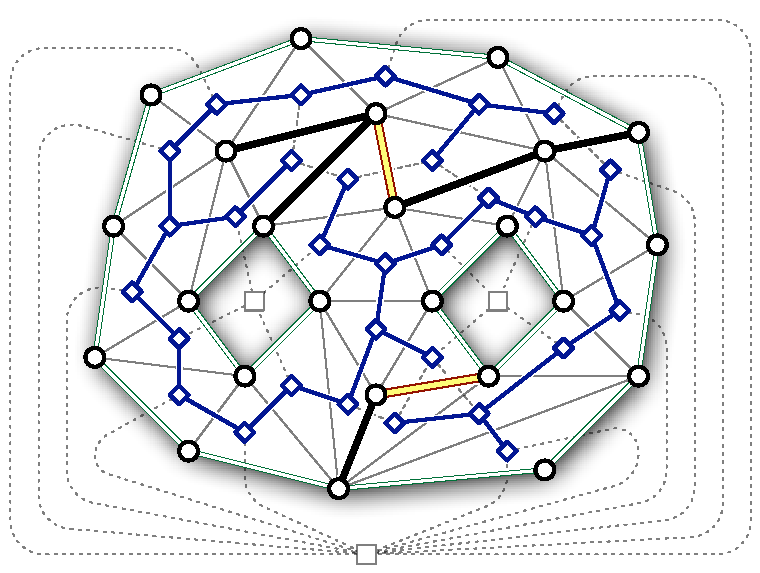
\includegraphics[scale=0.45]{Fig/forest-cotree2} \qquad
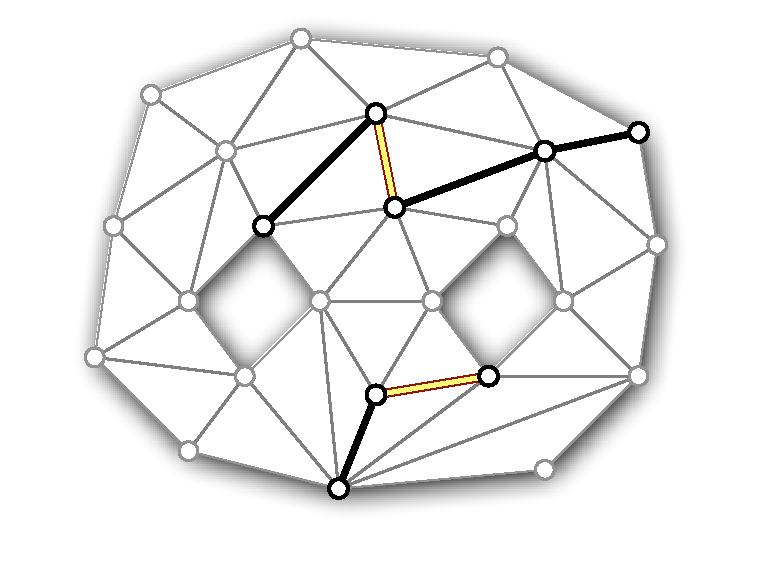
\includegraphics[scale=0.45]{Fig/forest-cotree-arcs2}
\end{tabular}
\caption{Left: A forest-cotree decomposition of the graph in Figure \ref{fig:duality}; thick doubled lines indicate edges in $X$.
Right: The resulting system of arcs.  Compare with Figure \ref{fig:tree-coforest}.}
\label{fig:forest-cotree}
\end{figure}

We can easily construct an \emph{arbitrary} forest-cotree decomposition in $O(n)$ time using whatever-first search, but we require a decomposition with a particular forest $F$.  Let $G/\partial G$ denote the graph obtained from $G$ by \emph{contracting} the entire subgraph $\partial G$---both vertices and edges---to a single vertex $x$.  Using the algorithm of Henzinger \etal~\cite{hkrs-fspap-97}
\note{Does Henzinger \etal\ work when we contract the boundaries? If not, how do we compute the primal tree in~$O(n \log \log n)$ time?}, we compute the single-source shortest-path tree $T$ in $G/\partial G$ rooted at $x$ in $O(n)$ time.  Let $F$ be the subgraph of $G$ corresponding to~$T$.  Each component of $F$ is a tree of shortest paths from a boundary vertex to a subset of the non-boundary vertices of $G$.  With the shortest-path forest $F$ in hand, we can easily construct the rest of the forest-cotree decomposition in $O(n)$ time.

Finally, for each edge $e_i\in X$, let $\sigma_i$ and $\tau_i$ denote the unique directed paths in $F$ from the boundary of~$G$ to the endpoints of $e_i$, and let $S := \set{\sigma\!_1, \dots, \sigma\!_\beta, \allowbreak \tau_1, \dots, \tau_\beta}$.  By construction of $F$, every element of~$S$ is a (possibly empty) shortest directed path.  Moreover, because $a_i = \sigma_i \cdot e_i \cdot \rev(\tau_i)$ for each index $i$, every non-null-homologous cycle in $G$ must intersect at least one path in $S$.  We can easily compute each path in $S$ in $O(n)$ time.

For any cycle $\gamma$ and any index $i$, let $x_i(\gamma)$ denote the number of times $\gamma$ crosses the arc~$a_i$.  The \EMPH{crossing vector} $x(\gamma)$ is the vector $(x_1(\gamma), \dots, x_\beta(\gamma))$.  The crossing vector of a set of cycles is the sum of the crossing vectors of its elements.
\begin{lemma}
\label{lem:decomposition}
Every even subgraph of an embedded graph has a cycle decomposition.
\end{lemma}

\begin{proof}
Let $H$ be an even subgraph of $G$.  We can decompose $H$ into cycles by specifying, at each vertex $v$, which pairs of incident edges of $H$ are consecutive.  Any pairing that does not create a crossing at $v$ is sufficient.  For example, if $e_1, e_2, \dots, e_{2d}$ are the edges of $H$ incident to $v$, indexed in clockwise order around $v$, we could pair edges $e_{2i-1}$ and $e_{2i}$ for each $i$.  
\end{proof}

Crossing vectors are not well-defined for arbitrary even subgraphs; different cycle decompositions can yield different crossing numbers.  However, the \emph{parity} of the crossing numbers is independent of the cycle decomposition.  The \EMPH{crossing parity vector} of any even subgraph $H$ is the bit vector $\bar{x}(H) = (\bar{x}_1, \dots, \bar{x}_\beta)$, where $\bar{x}_i = 1$ if the arc $a_i$ crosses (any cycle decomposition of) $H$ an odd number of times, and $\bar{x}_i = 0$ otherwise.

\begin{lemma}
Two even subgraphs are $\Z_2$-homologous if and only if their crossing parity vectors are equal.
\end{lemma}

\begin{proof}
Every boundary subgraph is the symmetric difference of facial cycles.  Any non-contractible loop or arc crosses any facial cycle an even number of times; thus, the crossing parity vector of any facial cycle is the zero vector.  Every pair of even subgraphs $H$ and $H'$ satisfies the identity $x(H\oplus H') = x(H) \oplus x(H')$.  Thus, the crossing parity vector of any boundary subgraph is the zero vector.
\end{proof}

\begin{lemma}
We can compute the crossing parity vector of any even subgraph in $O(\beta)$ time per edge after computing~$P$.
\end{lemma}

\begin{proof}
We can compute a cycle decomposition $\gamma_1, \dots, \gamma_r$ of $H$ in $O(1)$ time per edge, by following the proof of Lemma~\ref{lem:decomposition}.
We can compute the number of crossings between any cycle $\gamma_i$ and any arc $a_j$ in time proportional to the number of edges in $\gamma_i$.
\end{proof}



\subsection{Homology signatures}

Our second method associates a vector of $\beta$ bits with each edge $e$, called the \EMPH{signature} of~$e$; the homology class of any even subgraph is characterized by the bit-wise exclusive-or of the signatures of its edges.

Again, our construction is based on one of two natural generalizations of tree-cotree decompositions~\cite{e-dgteg-03} to surfaces with boundary; the other generalization is used for computing crossing parity vectors as described above and is used in Section \ref{sec:homcover}.
We define a \EMPH{tree-coforest decomposition} of $G$ to be any partition $(T, F, X)$ of the edges of $G$ into three edge-disjoint subgraphs with the following properties:
\begin{itemize}\itemsep0pt
\item $T$ is a spanning tree of $G$.
\item $F^*$ is a spanning \emph{forest} of $G^*$, that is, an acyclic subgraph that contains every vertex.
\item Each component of $F^*$ contains a single dual boundary vertex $\delta_i^*$.
\end{itemize}
Euler's formula implies that there are exactly $\beta$ edges in $X$; arbitrarily index these edges $e_1, \dots, e_\beta$.  For each edge $e_i\in X$, adding the corresponding dual edge $e_i^*$ to $F^*$ creates a new dual path $\dualarc_i$, which is either a simple path between distinct boundary vertices, or a nontrivial loop from a boundary vertex back to itself; in the second case, $\dualarc_i$ may traverse some edges of $F^*$ twice.  We can treat each path $\dualarc_i$ as a simple arc in the \emph{abstract} surface $\Sigma$; cutting along these $\beta$ arcs transforms $\Sigma$ into a topological disk.
See Figure \ref{fig:tree-coforest}.

\begin{figure}[htb]
\centering\footnotesize\sf
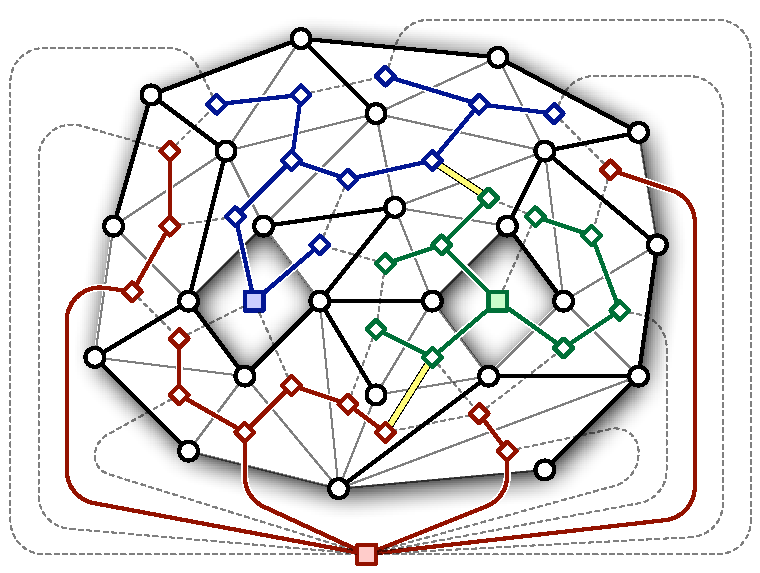
\includegraphics[scale=0.45]{Fig/tree-coforest2} \qquad
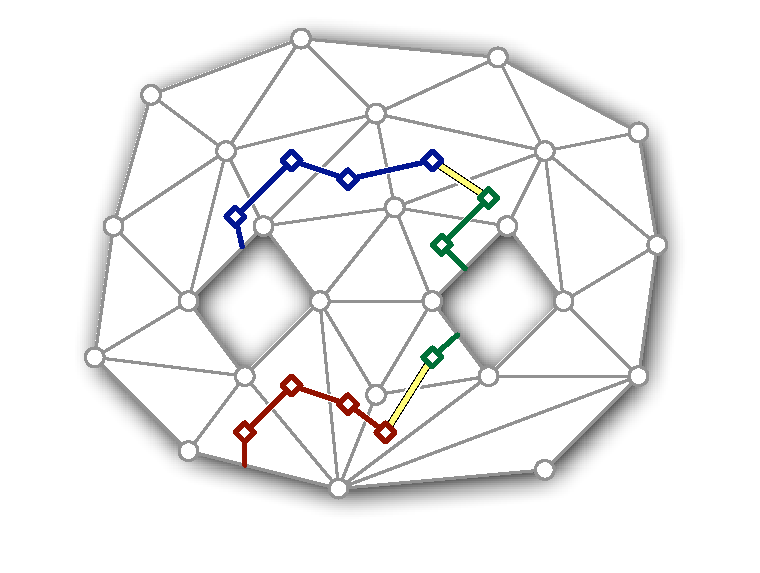
\includegraphics[scale=0.45]{Fig/tree-coforest-arcs2}
\caption{Left: A tree-coforest decomposition of the graph in Figure~\ref{fig:duality}; doubled lines indicate edges in $X$.
Right: The resulting system of dual arcs.  Compare with Figure \ref{fig:forest-cotree}.}
\label{fig:tree-coforest}
\end{figure}

Finally, for each edge $e$ in $G$, we define its signature \EMPH{$[e]$} to be the $\beta$-bit vector whose $i$th bit is equal to $1$ if and only if $e$ crosses $\dualarc_i$ (that is, if $\dualarc_i$ traverses the dual edge $e^*$) exactly once.  The signature $[\eta]$ of an even subgraph $\eta$ is the bitwise exclusive-or of the signatures of its edges.  Similarly, the signature~$[\cycle]$ of a cycle $\cycle$ is the bitwise exclusive-or of the signatures of the edges that $\cycle$ traverses an odd number of times.

Let \EMPH{$h \oplus h'$} denote the bitwise exclusive-or of two homology signatures $h$ and $h'$, or equivalently, their sum as elements of the homology group~$(\Z_2)^\beta$.  The identities $[\eta \oplus \eta'] = [\eta] \oplus [\eta']$ and $[\cycle\cdot\cycle'] = [\cycle] \oplus [\cycle']$ follow directly from the definitions.

\begin{lemma}
\label{lem:sign}
We can preprocess $G$ in $O(\beta n)$ time, so that the signature $[\cycle]$ of any cycle can be computed in $O(\beta)$ time per edge.
\end{lemma}

\begin{proof}
A tree-coforest decomposition can be computed in $O(n)$ time as follows.  First construct a graph~$H$ by identifying all the dual boundary vertices in $G^*$ to a single vertex.  Compute a spanning tree of $H$ by whatever-first search; the edges of this spanning tree define an appropriate dual spanning forest~$F^*$.  Construct the subgraph $G\setminus F$ and compute a spanning tree $T$ via whatever-first search.  Finally, let $X = G\setminus (T\cup F)$.  With the decomposition in hand, it is straightforward to compute each path $\dualarc_i$ in $O(n)$ time, and then compute each edge signature in $O(\beta)$ time.
\end{proof}

\begin{lemma}
An even subgraph $\eta$ of $G$ is null-homologous in $\Sigma$ if and only if $[\eta] = 0$.
\end{lemma}

\begin{proof}
Let $\eta$ be a null-homologous even subgraph of $G$.  Then by definition, $\eta$ is the boundary of the union of a subset~$Y$ of faces of $G$.  The boundary of any face $f$ is contractible in $\Sigma$ and therefore has signature $0$.  It follows immediately that $[\eta] = [\bigoplus_{f\in Y} \partial f] = \bigoplus_{f\in Y} [\partial f] = 0$.

Conversely, suppose $\eta$ crosses each arc $\dualarc_i$ an even number of times, so $[\eta]=0$.  Let $x$ and $y$ be two intersection points between $\eta$ and some arc $\dualarc_i$, and let $\dualarc_i[x,y]$ be the subpath of $\dualarc_i$ between those two points.  Replacing tiny segments of $\eta$ through~$x$ and~$y$ with two copies of $\dualarc_i[x,y]$ does not change the homology class of $\eta$, but does reduce the number of intersection points between $\eta$ and $\dualarc_i$.  It follows by induction that~$\eta$ is homologous to another even graph $\eta'$ that does not intersect any path~$\dualarc_i$ at all.  This even graph lies entirely within the disk $\Sigma\setminus \bigcup_i\dualarc_i$, and is therefore null-homologous.
\end{proof}


The following corollaries are now immediate.

\begin{corollary}
Two even subgraphs $\eta$ and $\eta'$ of $G$ are $\Z_2$-homologous in $\Sigma$ if and only if $[\eta] = [\eta']$.
\end{corollary}

\begin{corollary}
Two cycles $\cycle$ and $\cycle'$ in $G$ are $\Z_2$-homologous in $\Sigma$ if and only if $[\cycle] = [\cycle']$.
\end{corollary}
